\documentclass{article}

\usepackage[utf8]{inputenc}
\usepackage[T1]{fontenc}
\usepackage{a4wide}
\usepackage[french]{babel}
\usepackage[babel=true]{csquotes}
\usepackage{graphicx}
\graphicspath{{Images/}}
\usepackage{color}
\usepackage{hyperref}
\usepackage[top=1.5cm,bottom=1.5cm,right=1.5cm,left=1.5cm]{geometry}
\usepackage[nottoc,numbib]{tocbibind}
\hypersetup{colorlinks,linkcolor=,urlcolor=blue}

\usepackage{amsmath}
\usepackage{amssymb}
\usepackage{listings}

\usepackage{fancyhdr}
\pagestyle{fancy}
\renewcommand\headrulewidth{1pt}
\fancyhead[C]{Rapport de projet}
\fancyhead[L]{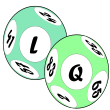
\includegraphics[scale=0.3]{dessin_logo_app_fond_chiffres110x110_sansFond.png}}
\fancyhead[R]{Université de La Réunion}
\renewcommand{\footrulewidth}{1pt}

\renewcommand{\footruleskip}{1pt}
\fancyfoot[C]{\thepage}
\fancyfoot[L]{\LaTeX}
\fancyfoot[R]{\today}


\title{Rapport de projet de développement d'une application mobile : LotoQuinote}
\author{David Boisedu et Alexandre Boyer}
\date{\today}

\begin{document}
\renewcommand{\textheight}{695pt}

\maketitle

\begin{abstract}
\begin{center}
L'application que nous avons développée répond à la problématique suivante : 
\newline \textit{Comment faciliter le suivi de tirage des numéros d'un loto-quine grâce à une application mobile ?}
\end{center}
\end{abstract}

\vspace{10em}
\renewcommand{\contentsname}{Sommaire}
\tableofcontents

\newpage

\section{Introduction}
\label{section:intro}

Cela peut être parfois fastidieux de noter sur une feuille tous les numéros sortis lors d'un tirage de loto-quine. C'est pour cette raison précise que nous avons décidé de créer une application qui faciliterai cette tâche. En plus de permettre de suivre le tirage d'un loto-quine, l'application LotoQuinote permet aussi d'enregistrer chaque tirage pour pouvoir les consulter à n'importe quel moment. De plus, grâce à des fonctions de tri, il est possible de voir très rapidement les numéros qui ont été tirés lors d'un tirage.

\section{Description générale de l'application LotoQuinote}

L'application LotoQuinote comporte trois vues :

\begin{itemize}
\vspace{1em}
    \item {\underline {\large{La vue d'accueil :}}}
\end{itemize} 
    \noindent%
    \begin{minipage}{.6\textwidth}%
    Cette vue permet la création d'un nouveau suivi de tirage et affiche tous les suivis de tirage crées sous forme d'une liste pouvant être défilée. 
    \end{minipage}%
    \hfill
    \begin{minipage}{.35\textwidth}%
        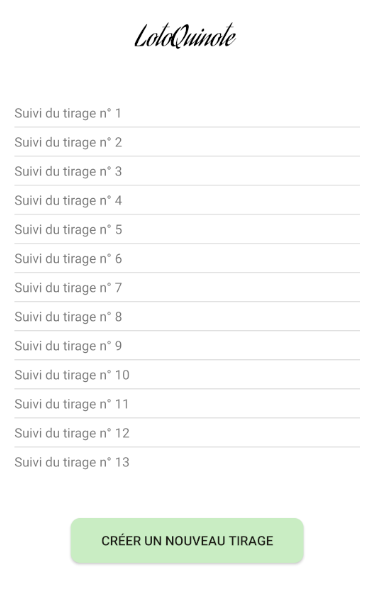
\includegraphics[scale=0.7]{accueil.png}
    \end{minipage}%
    
    \begin{minipage}{.35\textwidth}%
        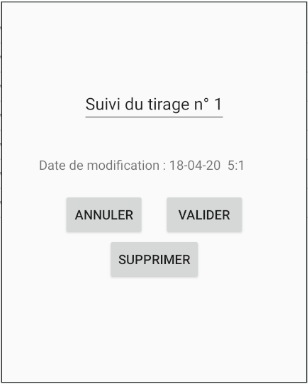
\includegraphics[scale=0.7]{edition.png}
    \end{minipage}%
    \hfill
    \begin{minipage}{.6\textwidth}%
    La vue d'accueil possède aussi une fonctionnalité d'édition lors d'un appui-long sur un suivi de tirage. Cette fonctionnalité permet de :
    \vspace{1em}
    \begin{itemize}
        \item Mofidier le titre du suivi de tirage
        \item Afficher la date de dernière modification
        \item Supprimer le suivi de tirage
    \end{itemize}
    \end{minipage}%
\vspace{4em}
\begin{itemize}
    \item {\underline{\large{La vue de suivi de tirage :}}}
\end{itemize}
\vspace{1em}
    \begin{minipage}{.6\textwidth}%
    La vue de suivi de tirage permet de choisir le numéro qui a été tiré lors du tirage du loto-quine. Le numéro est choisit soit par le biais du NumberPicker ou soit en l'écrivant soi-même grâce à l'EditText.
    \vspace{1em}
    \newline
    Lors du clique sur le bouton "Ajouter", le numéro choisit est inséré à la liste des numéros tirés. Les cinq derniers numéros tirés de cette liste sont visibles dans les cases situées en bas de cette vue.
    \vspace{1em}
    \newline Le bouton "Terminer" permet de sauvegarder les numéros ajoutés à la liste et de revenir à la vue d'accueil.
    \vspace{1em}
    \newline
    La croix située en-dessous de la 1ère case à gauche permet de supprimer le dernier numéro ajouté à la liste.
    \vspace{1em}
    \newline
    Le bouton "+" à droite de la dernière case permet de basculer sur la vue de la liste complète des numéros tirés. 
    \end{minipage}%
    \hfill
    \begin{minipage}{.35\textwidth}%
        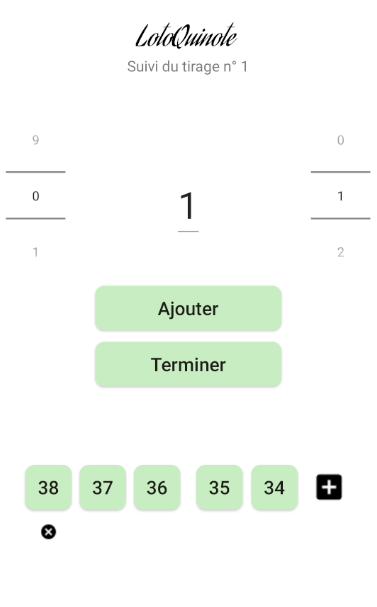
\includegraphics[scale=0.7]{suivi.png}
    \end{minipage}%
\vspace{2em}
\newline
\underline{Remarque :}  A chaque ajout d'un numéro à la liste, un toast nous informe que celui-ci a bien été ajouté. Si le numéro que l'on veut ajouter est déjà présent dans la liste un toast apparaît pour signaler le fait que ce numéro a déjà été tiré et qu'il ne sera donc pas ajouté.
\newpage
\begin{itemize}
    \item {\underline{\large{La vue de la liste des numéros tirés :}}}
\end{itemize}
\vspace{1em}
    \begin{minipage}{.35\textwidth}%
        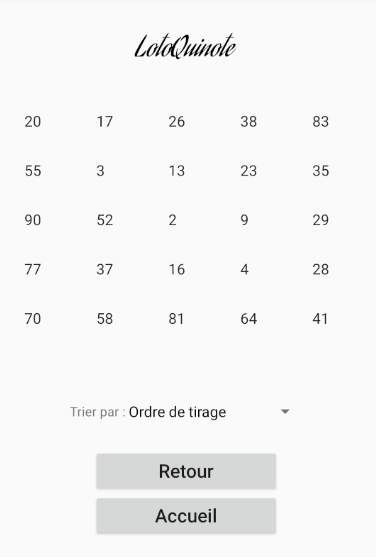
\includegraphics[scale=0.7]{liste.png}
    \end{minipage}%
    \hfill
    \begin{minipage}{.6\textwidth}%
    Cette vue permet de voir l'ensemble des numéros tirés lors du tirage du loto-quine. Par défaut, les numéros sont triés par ordre de tirage : le dernier numéro tiré est le premier de la liste.
    \vspace{1em}
    \newline
    D'autres fonctions de tri sont disponibles par le biais d'une petite liste déroulante. On peut ainsi trier les numéros par :
    \begin{itemize}
        \item Ordre de tirage
        \item Ordre croissant
        \item Ordre décroissant
    \end{itemize}
    \end{minipage}%
    
    
    


\section{Architecture du code}


    \begin{minipage}{.6\textwidth}%
    Le code de notre application suit l'architecture MVC \newline (Modèle, Vue, Contrôleur).
    \vspace{1em}
    \newline Ainsi, la partie "Contrôleur" contient les activités principales de notre application.
    \vspace{1em}
    \newline La partie "Modèle" contient les classes que nous utilisons pour définir les objets nécessaires à notre application.
    \vspace{1em}
    \newline Et la partie "Vue" représenté par le dossier "layout" contient les fichiers .xml qui permettent l'interaction entre l'application et l'utilisateur. 
    \end{minipage}%
    \hfill
    \begin{minipage}{.35\textwidth}%
        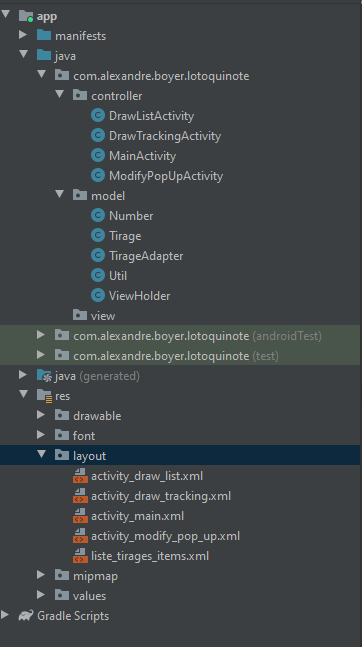
\includegraphics[scale=0.6]{archiMVC.png}
    \end{minipage}%

\newpage
\subsection{La partie "Contrôleur" de l'application}
\subsubsection{MainActivity}
\vspace{1em}
\underline{Le code de MainActivity est construit en suivant cette architecture :}
\vspace{1em}
\newline Tout d'abord, la liste qui va contenir les tirages est crée par le biais de la classe objet "TirageAdapter" :
\newline
\begin{center} 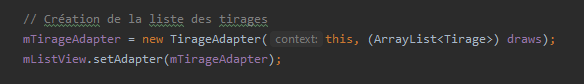
\includegraphics[]{creationList_mainActivity.png} \end{center}
\vspace{1em}
Ensuite, une écoute sur le bouton "Créer un nouveau tirage" est réalisé pour permettre la création d'un tirage lors de l'appui sur celui-ci. Un toast est aussi crée lors de l'appui pour signaler la création d'un nouveau tirage :
\newline
\begin{center} 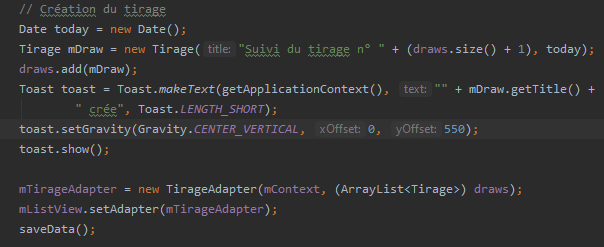
\includegraphics[]{creationTirage_mainActivity.png} \end{center}
\vspace{1em}
Un délai a été mis en place sur ce bouton pour qu'on puisse l'actionner qu'une fois toute les deux secondes, cela pour éviter de spammer la création de tirages :
\newline
\begin{center} 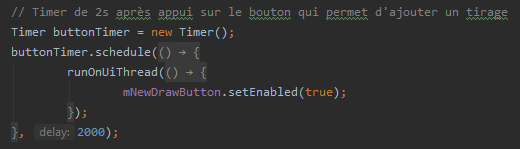
\includegraphics[]{timer_MainActivity.png} \end{center}
\vspace{1em}
De la même manière, une écoute sur les items de la liste est réalisée pour pouvoir changer d'activité lors de l'appui. Ainsi, si l'utilisateur appui sur un tirage de la liste, il sera dirigé vers la vue de suivi de tirage (DrawTrackingActivity).
\vspace{1em}
\newline Il en est de même pour la gestion de l'appui long sur un tirage : lorsque l'utilisateur réalise un appui long sur un tirage de la liste, une fenêtre d'édition apparaît comme expliqué plus haut.
\vspace{1em}
\newline Enfin, la dernière partie du code de MainActivity concerne la sauvegarde des données qui se fait dans notre cas grâce aux SharedPreferences~\cite{sharedPreferences}.

\newpage
\subsubsection{DrawTrackingActivity}
\vspace{1em}
\underline{Le code de DrawTrackingActivity est construit en suivant cette architecture :}
\vspace{1em}
\newline Au début de cette activité, nous récupérons le titre du tirage depuis MainActivity pour l'afficher sur la vue de DrawTrackingActivity grâce la classe Intent~\cite{intent} :
\newline
\begin{center} 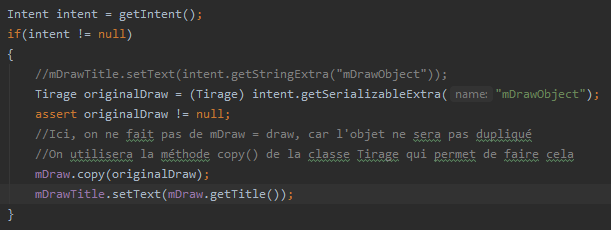
\includegraphics[scale=0.8]{intent_DrawTrackingActivity.png} \end{center}
\vspace{1em}
Dans la suite du code, nous gérons les interactions avec les différents éléments présents sur cette activité. Par exemple, nous avons codé le fonctionnement des NumberPickers pour qu'ils répondent aux besoins d'une application qui permet le suivi du tirage d'un loto-quine et donc par conséquent des numéros qui doivent être compris entre 0 et 90 :
\newline
\begin{center} 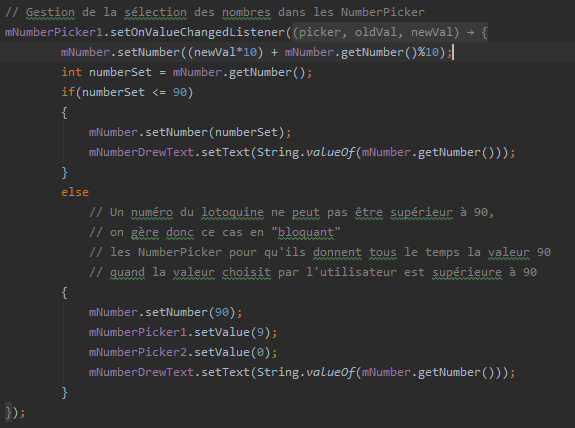
\includegraphics[scale=0.8]{numberPicker_DrawTrackingActivity.png} \end{center}
\vspace{1em}
La gestion de l'ajout et de la suppression des numéros à la liste de tirage constitue la dernière partie du code de DrawTrackingActivity. Ainsi, dans cette partie du code, grâce à un listener sur le bouton "Ajouter", on ajoute le numéro choisit à la liste en fonction de s'il a déjà été tiré ou non. De plus, on gère aussi l'affichage des cinq derniers numéros tirés dans les cases situées en bas de cette activité. Cette gestion de l'affichage se fait à l'aide d'un switch qui se base sur la taille de la liste.
\newpage
\begin{center} 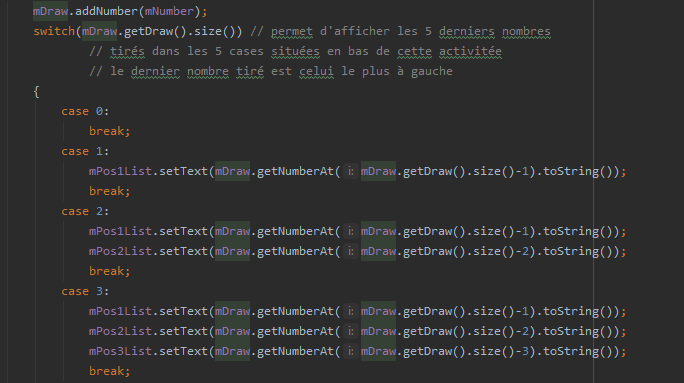
\includegraphics[]{switch_DrawTrackingActivity.png} \end{center}
Dans ce switch, la position des numéros dans les cases change en fonction du nombre de numéros pour que le dernier numéro tiré soit tous le temps celui le plus à gauche.
\vspace{1em}
\newline La gestion de la suppression du dernier numéro tiré par le biais de l'ImageButton représentant une petite croix se fait de la même manière que lors de l'ajout d'un numéro, sauf qu'ici, au lieu d'ajouter un numéro de la liste, on l'enlève de cette liste :
\newline
\begin{center} 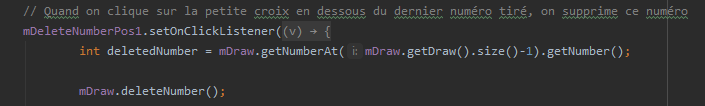
\includegraphics[]{delete_DrawTrackingActivity.png} \end{center}
\vspace{1em}
Enfin, l'appui sur le bouton "+" permet de lancer la troisième et dernière activité de notre application, DrawListActivity. Se faisant, on récupère aussi tous les numéros ajoutés à la liste grâce à ces deux lignes de code : 
\begin{lstlisting}
    Intent drawListActivity = new Intent(DrawTrackingActivity.this, DrawListActivity.class);
    drawListActivity.putExtra("drawList", mDraw);
\end{lstlisting}
Ainsi, ces deux lignes permettent de récupérer les données de l'activité courante pour les transférer à l'activité suivante.

\newpage
\subsubsection{DrawListActivity}
\vspace{1em}
\underline{Le code de DrawListActivity est construit en suivant cette architecture :}
\vspace{1em}
\newline Tout comme pour la DrawTrackingActivity, nous allons récupérer le tirage par le biais de la classe Intent :
\newline
\begin{center} 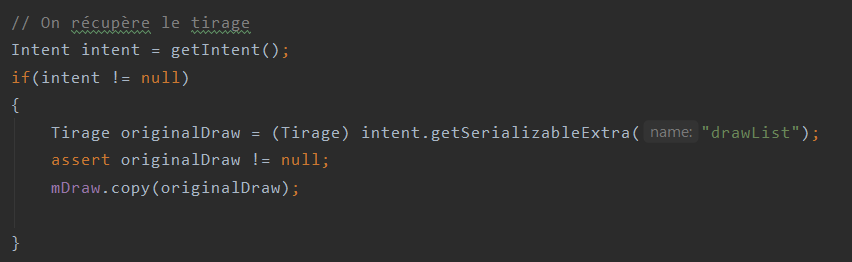
\includegraphics[scale=0.8]{intent_DrawListActivity.png} \end{center}
\vspace{1em}
Suite à cela, nous allons mettre en place un Spinner\cite{spinner}, qui va permettre à l'utilisateur de choisir la manière dont les numéros sont triés pour les afficher :
\begin{center} 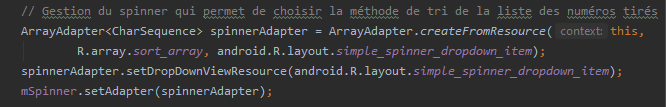
\includegraphics[scale=0.7]{spinner_DrawListActivity.png} \end{center}
Enfin, le comportement de notre Spinner va être géré par la structure de contrôle switch. Chacun des "cases" sera lié à un élément de notre Spinner, et va permettre à l'utilisateur de choisir le mode de tri des numéros, et ainsi changer l'affichage.
\newline Les affichages sont gérés par la création d'un ArrayAdapter\cite{arrayAdapter} sur notre élément graphique GridView\cite{gridview} :
\begin{center} 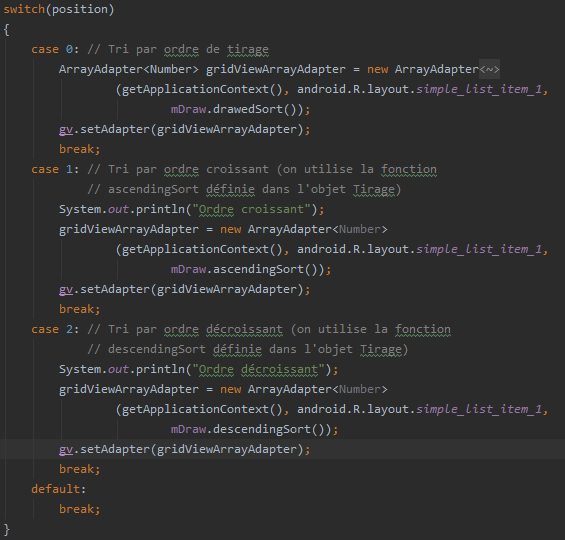
\includegraphics[scale=0.8]{switch_DrawListActivity.png} \end{center}

\newpage
\subsubsection{ModifyPopUpActivity}
\noindent Cette activité permet la gestion de l'interface d'édition qui apparaît lors de l'appui long sur un tirage de la vue d'accueil.
\newline Le code de cette activité se décompose comme cela :
\vspace{1em}
\newline On récupère encore une fois les données du tirage grâce à un Intent :
\vspace{1em}
\newline
\begin{center} 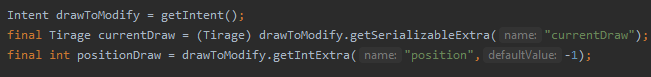
\includegraphics[]{intent_popUpAct.png} \end{center}
\vspace{1em}
On met à jour les éléments graphiques de la vue avec les données récupérées par l'Intent :
\newline
\begin{center} 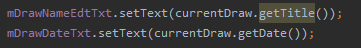
\includegraphics[]{maj_popUpAct.png} \end{center}
\vspace{1em}
On gère ensuite les interactions avec les différents boutons présents sur cette activité :
\vspace{1em}
\newline
\begin{center} 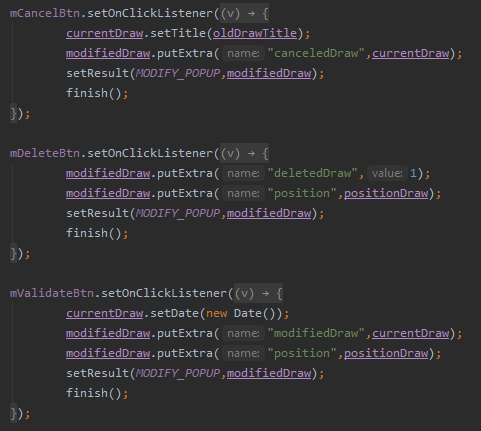
\includegraphics[]{interactions_popUpAct.png} \end{center}

\newpage
\subsection{La partie "Modèle" de l'application}
L'application LotoQuinote se base sur 3 principaux modèles :
\subsubsection{La classe "Number"}
Cette classe permet de définir l'objet Number qui est l'un des objets indispensables de notre application.
\newline Celle-ci implémente les interfaces Serializable\cite{serializable} et Comparable\cite{comparable} pour pouvoir respectivement utiliser la classe Intent et comparer les objets Number entre eux.
\newline La classe Objet dispose de Getter/Setter simples, d'une méthode toString() qui convertit un objet Number en chaîne de caractères et d'une méthode compareTo() liée à l'interface Comparable.

\subsubsection{La classe "Tirage"}
Cette classe définit l'objet Tirage. Cet objet est au coeur de notre application puisque c'est sur lui que repose le principe de suivi de tirage. Lui aussi implémente l'interface Serializable qui permet l'utilisation de l'Intent.
\newline Cette classe possède trois attributs :
\begin{itemize}
    \item Un titre
    \item Une date
    \item Un ArrayList d'objets Number
\end{itemize}
Elle possède des getter/setter pour chacun de ces attributs ainsi que des méthodes supplémentaires utiles dans les différentes activités de l'application, comme notamment les méthodes de tri :
\vspace{1em}
\newline
\begin{center}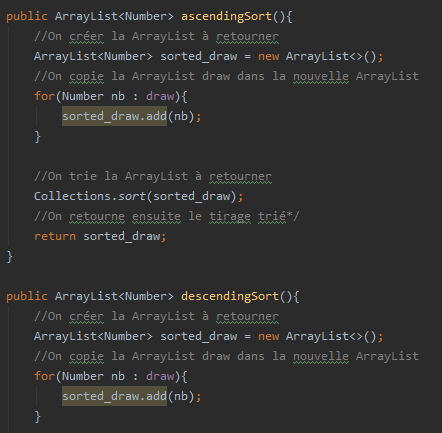
\includegraphics[]{tri_Tirage.png}\end{center}

\subsubsection{La classe "TirageAdapter"}
Cette classe définit l'objet TirageAdapter. Elle prend en paramètre un ArrayList d'objets Tirage et possède différentes méthodes qui permettent de gérer la liste des tirages de l'application LotoQuinote.


\section{Quelques points délicats/intéressants}
\subsection{Choix de la méthode d'édition et de suppression des tirages}
\vspace{1em}
Au tout début du projet, concernant l'activité "MainActivity", nous avions pour objectif de gérer la modification/suppression des différents tirages par le biais de CheckBox. En effet, elles auraient permis de choisir le ou les tirages à modifier/supprimer, puis par le biais d'icônes, de réaliser l'action souhaité.
\newline Malheureusement, cela nous a pris beaucoup de temps sur notre projet ainsi que beaucoup de bugs à la chaîne. Nous avons donc pris le choix d'abandonner cette idée et de partir sur la création d'une nouvelle activité permettant la modification/suppression d'un tirage, se manifestant sous la forme d'une Pop-Up.

\section{Conclusion}
\vspace{1em}
La réalisation de ce projet s'est plutôt bien déroulé. Nous avons pu réaliser ce que nous souhaitions, c'est-à-dire, une application permettant la sauvegarde de tirages d'un loto-quine. Malgré les difficultés rencontrées, nous avons également réussis à respecter les consignes imposées, cela grâce à une bonne entente et une bonne organisation du travail.
\newline Nous pensons que ce projet peut encore s'étendre, notamment avec l'implémentation de paramètres de personnalisation de l'interface, la gestion des joueurs ( sauvegarde des noms, nombres de victoires, etc ... ), et des gains.


\newpage

\begin{thebibliography}{}

\bibitem{sharedPreferences}
Tutos android, \textit{SharedPreferences} : \url{http://tutos-android-france.com/sharedpreferences-2/}

\bibitem{intent}
Android Developers, Intent Class : \url{https://developer.android.com/reference/android/content/Intent}

\bibitem{spinner}
Android Developers, \textit{Spinners} :
\url{https://developer.android.com/guide/topics/ui/controls/spinner}

\bibitem{arrayAdapter}
Medium, \textit{Array Adpaters} : \url{https://medium.com/mindorks/custom-array-adapters-made-easy-b6c4930560dd}

\bibitem{gridview}
Android Developers, \textit{GridView} :
\url{https://developer.android.com/reference/android/widget/GridView}

\bibitem{serializable}
Android Developers, \textit{Serializable} :
\url{https://developer.android.com/reference/java/io/Serializable}

\bibitem{comparable}
Android Developers, \textit{Comparable} :
\url{https://developer.android.com/reference/java/lang/Comparable}

\end{thebibliography}

\end{document}
